\tikzset{p_style/.style={circle, fill=green!20, minimum size=0.2cm}}
\subfigure[Concrete symbols]
{
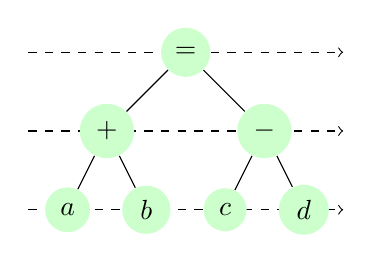
\begin{tikzpicture}
    \draw[->, dashed] (-2,0) -- (2,0);
    \draw[->, dashed] (-2,-1) -- (2,-1);
    \draw[->, dashed] (-2,-2) -- (2,-2);

    \node[p_style] (=) at (0,0){$=$};
    \node[p_style] (+) at (-1,-1){$+$};
    \node[p_style] (-) at (1,-1){$-$};
    \node[p_style] (a) at (-1.5, -2) {$a$};
    \node[p_style] (b) at (-0.5, -2) {$b$};
    \node[p_style] (c) at (0.5, -2) {$c$};
    \node[p_style] (d) at (1.5, -2) {$d$};

    \draw[] (=) -- (+);
    \draw[] (=) -- (-);
    \draw[] (+) -- (a);
    \draw[] (+) -- (b);
    \draw[] (-) -- (c);
    \draw[] (-) -- (d);
    
\end{tikzpicture}
}
\subfigure[Positonal encoding]
{
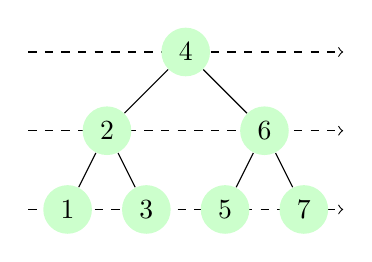
\begin{tikzpicture}
    \draw[->, dashed] (-2,0) -- (2,0);
    \draw[->, dashed] (-2,-1) -- (2,-1);
    \draw[->, dashed] (-2,-2) -- (2,-2);

    \node[p_style] (=) at (0,0){$4$};
    \node[p_style] (+) at (-1,-1){$2$};
    \node[p_style] (-) at (1,-1){$6$};
    \node[p_style] (a) at (-1.5, -2) {$1$};
    \node[p_style] (b) at (-0.5, -2) {$3$};
    \node[p_style] (c) at (0.5, -2) {$5$};
    \node[p_style] (d) at (1.5, -2) {$7$};

    \draw[] (=) -- (+);
    \draw[] (=) -- (-);
    \draw[] (+) -- (a);
    \draw[] (+) -- (b);
    \draw[] (-) -- (c);
    \draw[] (-) -- (d);
    
\end{tikzpicture}
}
\subfigure[Shifted positonal encoding]
{
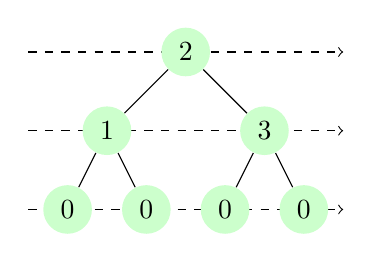
\begin{tikzpicture}
    \draw[->, dashed] (-2,0) -- (2,0);
    \draw[->, dashed] (-2,-1) -- (2,-1);
    \draw[->, dashed] (-2,-2) -- (2,-2);

    \node[p_style] (=) at (0,0){$2$};
    \node[p_style] (+) at (-1,-1){$1$};
    \node[p_style] (-) at (1,-1){$3$};
    \node[p_style] (a) at (-1.5, -2) {$0$};
    \node[p_style] (b) at (-0.5, -2) {$0$};
    \node[p_style] (c) at (0.5, -2) {$0$};
    \node[p_style] (d) at (1.5, -2) {$0$};

    \draw[] (=) -- (+);
    \draw[] (=) -- (-);
    \draw[] (+) -- (a);
    \draw[] (+) -- (b);
    \draw[] (-) -- (c);
    \draw[] (-) -- (d);
    
\end{tikzpicture}
}
\caption{
    Sub-figure (a) shows the example term $a+b=c-d$ as a syntax tree.
    When you count the nodes from left to right, you get the positions in (b).
    By dividing each even position by the spread $s=2$ and discarding the non-integer nodes, you get the shifted encodings, showed in sub-figure (c).
}
